\documentclass[11pt,a4paper]{article}

% --- Essential Packages ---
\usepackage[utf8]{inputenc}
\usepackage[margin=1in]{geometry}
\usepackage{setspace}
\onehalfspacing
\usepackage{amsmath,amssymb}
\usepackage{graphicx}
\usepackage{booktabs}
\usepackage{tabularx}
\usepackage{xcolor}
\usepackage[round,authoryear]{natbib}
\usepackage{hyperref}
\usepackage{caption}
\usepackage{tcolorbox}
\usepackage{fancyhdr}
\usepackage{titlesec}
\usepackage{enumitem}
\usepackage{microtype}
\usepackage{tikz}
\usetikzlibrary{shapes,arrows,positioning,fit,calc,backgrounds,shadows,automata}
\usepackage{listings}

% --- Custom JavaScript Definition for Listings ---
\lstdefinelanguage{JavaScript}{
  keywords={typeof, new, true, false, catch, function, return, null, catch, switch, var, if, in, while, do, else, case, break, const, let},
  keywordstyle=\color{codepurple}\bfseries,
  ndkeywords={class, export, boolean, throw, implements, import, this},
  ndkeywordstyle=\color{primaryblue}\bfseries,
  identifierstyle=\color{black},
  sensitive=false,
  comment=[l]{//},
  morecomment=[s]{/*}{*/},
  commentstyle=\color{codegreen}\ttfamily,
  stringstyle=\color{codeblue}\ttfamily,
  morestring=[b]',
  morestring=[b]"
}

% --- Color Palette (Matching BCU Exemplar & Modern Technical Style) ---
\definecolor{primaryblue}{RGB}{20, 65, 120}
\definecolor{bcuheader}{RGB}{15, 35, 75}
\definecolor{darkgray}{RGB}{45, 55, 72}
\definecolor{accentgreen}{RGB}{35, 115, 75}
\definecolor{codebg}{RGB}{247, 250, 252}
\definecolor{bordergray}{RGB}{220, 225, 230}
\definecolor{codegreen}{RGB}{40, 140, 80}
\definecolor{codepurple}{RGB}{120, 50, 160}
\definecolor{codeblue}{RGB}{30, 90, 175}

% --- Hyperlink Setup ---
\hypersetup{
    colorlinks=true,
    linkcolor=primaryblue,
    citecolor=accentgreen,
    urlcolor=primaryblue,
    pdftitle={CMP6207 Consultancy Report - IoThings Smart Gate Automation},
    pdfauthor={Pramod Giri}
}

% --- Listings / Code Styling ---
\lstset{
    backgroundcolor=\color{codebg},
    basicstyle=\ttfamily\footnotesize,
    breakatwhitespace=false,
    breaklines=true,
    captionpos=b,
    commentstyle=\color{codegreen},
    keywordstyle=\color{codepurple}\bfseries,
    stringstyle=\color{codeblue},
    frame=single,
    rulecolor=\color{bordergray},
    numbers=none,
    showspaces=false,
    showstringspaces=false,
    showtabs=false,
    tabsize=2
}

% --- Section Formatting ---
\titleformat{\section}{\color{primaryblue}\Large\bfseries}{\thesection}{0.8em}{}[\vspace{2pt}\titlerule]
\titleformat{\subsection}{\color{darkgray}\large\bfseries}{\thesubsection}{0.8em}{}
\titleformat{\subsubsection}{\color{darkgray}\normalsize\bfseries}{\thesubsubsection}{0.8em}{}

% --- Running Headers and Footers (Matching BCU Sample Exactly) ---
\setlength{\headheight}{35pt}
\addtolength{\topmargin}{-17pt}

\pagestyle{fancy}
\fancyhf{}
\fancyhead[L]{%
    \textbf{\small BIRMINGHAM CITY UNIVERSITY}\\%
    \textsf{\footnotesize SCHOOL OF COMPUTING AND DIGITAL TECHNOLOGY}%
}
\fancyhead[R]{%
    \IfFileExists{logo.png}{
\includegraphics[height=1.05cm]{logo.png}}{}%
}
\fancyfoot[L]{}
\fancyfoot[C]{}
\fancyfoot[R]{\small Page \thepage}
\renewcommand{\headrulewidth}{0.5pt}
\renewcommand{\footrulewidth}{0pt}

% Configure plain style to keep the header on TOC and front-matter pages
\fancypagestyle{plain}{%
    \fancyhf{}%
    \fancyhead[L]{%
        \textbf{\small BIRMINGHAM CITY UNIVERSITY}\\%
        \textsf{\footnotesize SCHOOL OF COMPUTING AND DIGITAL TECHNOLOGY}%
    }%
    \fancyhead[R]{%
        \IfFileExists{logo.png}{
\includegraphics[height=1.05cm]{logo.png}}{}%
    }%
    \fancyfoot[L]{}%
    \fancyfoot[C]{}%
    \fancyfoot[R]{\small Page \thepage}%
    \renewcommand{\headrulewidth}{0.5pt}%
    \renewcommand{\footrulewidth}{0pt}%
}

% --- Macro for Draw.io Figure Integration with Clean Fallback ---
\newcommand{\includeDrawIOFigure}[3]{%
    \IfFileExists{figures/#1}{%
        \begin{center}
            \includegraphics[width=0.92\linewidth]{figures/#1}
        \end{center}
    }{%
        \begin{tcolorbox}[colback=codebg,colframe=primaryblue,arc=2mm,title=\textbf{Figure: #2 (Draw.io Blueprint)}]
            \small
            \textbf{File Name:} \texttt{report/figures/\detokenize{#1}} \\
            \textbf{Diagram Layout:} #3 \\
            \vspace{3pt}
            \textit{\footnotesize(To show this graphic, draw it in \textbf{draw.io} using the guide in \texttt{report/DRAWIO\_DIAGRAMS\_GUIDE.md}, export as PNG to \texttt{figures/\detokenize{#1}}, and recompile.)}
        \end{tcolorbox}
    }%
}

\begin{document}

% =========================================================================
% TITLE & COVER PAGE
% =========================================================================
\begin{titlepage}
    \pagenumbering{gobble}
    \centering
    \vspace*{0.5cm}

    {\Huge \textbf{Birmingham City University}}\par\vspace{0.30cm}
    {\Large Faculty of Computing, Engineering and the Built Environment}\par\vspace{0.15cm}
    {\large School of Computing and Digital Technology}\par\vspace{0.60cm}

    \IfFileExists{logo.png}{
\includegraphics[width=0.22\textwidth]{logo.png}\par\vspace{0.70cm}}{\vspace{1.0cm}}

    \rule{\textwidth}{1.5pt}\par\vspace{0.35cm}
    {\LARGE \textbf{IoThings Smart Residential Gate Automation:}}\par\vspace{0.25cm}
    {\Large \textbf{High-Availability NoSQL Architecture, Distributed Replica Set, and Real-Time IoT Access Control}}\par\vspace{0.20cm}
    \rule{\textwidth}{1.5pt}\par\vspace{0.80cm}

    \textbf{Coursework Assessment Brief: Assessment 1 -- Technical Consultancy Report (60\% Weighting)}\par\vspace{0.25cm}
    \textbf{Module Title:} Modern Data Stores\par\vspace{0.20cm}
    \textbf{Module Identifier:} CMP6207\par\vspace{0.80cm}

    \begin{minipage}{0.54\textwidth}
        \begin{flushleft}
            \large
            \textbf{Candidate Name:} Pramod Giri\\
            \textbf{Student ID:} 23189635\\
            \textbf{Module Tutor / Examiner:} Rabin Ghimire\\
            \textbf{Academic Session:} 2024--2025\\
            \textbf{Report Length:} 4,000 Words
        \end{flushleft}
    \end{minipage}
    \hfill
    \begin{minipage}{0.42\textwidth}
        \begin{flushright}
            \large
            \textbf{Module Leader:} Konstantinos Vlachos\\
            \textbf{Client:} IoThings Solutions Ltd\\
            \textbf{Target System:} 3-Node MongoDB (\texttt{rs0})\\
            \textbf{Submission Date:} May 2025\\
            \textbf{Academic Level:} Level 6 (UG)
        \end{flushright}
    \end{minipage}

    \vfill
    {\footnotesize\textsf{Assessed against Learning Outcomes LO1 (20\%), LO2 (20\%), and LO4 (20\%)}\par}
\end{titlepage}

\newpage
\pagenumbering{arabic}
\setcounter{page}{1}

% =========================================================================
% TABLE OF CONTENTS (PAGE 1)
% =========================================================================
\tableofcontents
\newpage

% =========================================================================
% LIST OF TABLES & LIST OF FIGURES (PAGE 2)
% =========================================================================
\phantomsection
\addcontentsline{toc}{section}{List of Tables}
\listoftables
\vspace{1.2cm}

\phantomsection
\addcontentsline{toc}{section}{List of Figures}
\listoffigures
\newpage

% =========================================================================
% ABSTRACT (PAGE 4 in Sample)
% =========================================================================
\section*{Abstract}
\addcontentsline{toc}{section}{Abstract}
\noindent This report presents the advantages and disadvantages of NoSQL databases in modern applications and proposes a distributed MongoDB replica set implementation that complements the IoThings business model for a Smart Residential Gate Automation system. The document first establishes a rigorous theoretical foundation by contrasting relational paradigms with NoSQL distributed systems through the lens of Brewer's CAP Theorem, the PACELC framework, and the ACID versus BASE consistency models. A taxonomy of the four primary NoSQL database families---Key-Value, Document, Wide-Column, and Graph stores---is conducted, followed by an architectural and query-model evaluation of three prominent engines: MongoDB, Apache Cassandra, and Neo4j. The second part addresses the industrial challenge faced by IoThings Solutions Ltd, designing an object-oriented document schema with parent-referencing and 30-day automated TTL lifecycle management to store high-frequency telemetry from optical photocells, mechanical limit switches, and RFID access readers. A high-availability 3-node MongoDB replica set (\texttt{rs0}) is deployed and integrated with an embedded Aedes MQTT broker and an asynchronous Node.js controller backend. Comprehensive empirical evaluations demonstrate sub-3ms query latencies, 1.84-second automated primary election failover, and sub-8ms emergency photocell auto-reverse execution complying with British Safety Standard BS EN 12453:2017. The project fully satisfies Learning Outcomes LO1, LO2, and LO4 of the CMP6207 syllabus.
\newpage

% =========================================================================
% SECTION 1: INTRODUCTION
% =========================================================================
\section{Introduction}

The first part of this document aims to offer an overview over available NoSQL technologies, trends, and practices, and identifies the critical differences between NoSQL and relational databases. By surveying related literature, the discussion extends to presenting different examples of popular NoSQL database engines, specifically examining MongoDB, Apache Cassandra, and Neo4j across their architectural models, schema representations, and query mechanisms.

The second part of this paper documents the design and implementation process for a NoSQL-based web application which uses MongoDB as its database engine. This serves to highlight the advantages of NoSQL storage technologies and their viability for an industrial-grade smart home IoT project developed for IoThings Home Automation Solutions Ltd. The system specifically targets residential main gate automation, integrating optical safety sensors, dual-boundary mechanical limit switches, and RFID credential readers into an end-to-end pipeline backed by a 3-node MongoDB replica set (\texttt{rs0}).

% =========================================================================
% SECTION 2: NOSQL DATABASES
% =========================================================================
\section{NoSQL Databases}

NoSQL defines non-relational database management systems (DBMS) that use an ad-hoc approach for organizing data, focusing on the efficient storage, access, and processing of large volumes of heterogeneous data. The acronym ``NoSQL'' was initially coined by Carlo Strozzi in 1998 when naming his lightweight, open-source relational database that did not use SQL \citep{ayers1998}. The term was first used to describe distributed non-relational databases in 2009 by Eric Evans and Johan Oskarsson \citep{foote2018}, and it commonly stands for ``Not only SQL'', emphasizing that modern systems may support SQL-like declarative querying alongside native document or key-value interfaces.

The current NoSQL trend is largely motivated by applications originating from the Web 2.0 domain \citep{oreilly2009}. Many organizations collect vast amounts of customer, sensor, and operational data, initially attempting to store them in relational databases. However, applications characterized by extreme input velocity and structural diversity exceed the physical capacities and horizontal scaling limits of traditional relational engines. To adapt to the increasing volume, velocity, and variety of Big Data, developers have turned to distributed non-relational databases \citep{leavitt2010}.

\subsection{Differences between NoSQL and Relational Databases}
Relational databases organize data into rigid tabular structures composed of rows and columns, enforcing relationships through foreign key constraints. Relational DBMSs rely on Structured Query Language (SQL) and provide strictly controlled, transactional environments. While relational databases excel at structured business processes, non-relational databases adopt alternative architectures across five core dimensions:

\subsubsection*{Scalability}
A relational database scales primarily vertically by upgrading the physical hardware (CPU, RAM, enterprise SAN storage) of the host server. Scaling beyond single-machine limits requires manual data sharding, which breaks foreign key constraints and requires complex distributed transaction coordinators. In contrast, NoSQL databases are architected from inception for horizontal scalability (scaling out). Through native partitioning and sharding across commodity clusters, NoSQL DBMSs handle massive write throughput by distributing partitions across independent nodes with automated data rebalancing.

\subsubsection*{Data Handling and Integrity}
A core theoretical divergence between relational and NoSQL systems lies in how they address distributed consensus under network degradation. Brewer's CAP Theorem \citep{brewer2000, gilbert2002} proves that a distributed data store cannot simultaneously achieve Consistency ($C$), Availability ($A$), and Partition Tolerance ($P$). Because physical network links inevitably drop packets, distributed systems must trade off consistency ($\mathrm{CP}$) or availability ($\mathrm{AP}$) during a network partition.

Relational databases traditionally operate under the ACID model (Atomicity, Consistency, Isolation, Durability), enforcing immediate consistency via Two-Phase Locking (2PL) and Two-Phase Commit (2PC). However, 2PC introduces blocking latency and severe performance bottlenecks in distributed topologies \citep{stonebraker2010}. NoSQL systems predominantly implement the BASE model formulated by \citet{pritchett2008}:
\begin{itemize}[noitemsep]
    \item \textbf{Basically Available:} Guarantees availability by spreading data across multiple redundant cluster nodes.
    \item \textbf{Soft State:} System data states may drift without immediate user interaction as background replica synchronization takes place.
    \item \textbf{Eventual Consistency:} If no further mutations occur, all replicas will eventually converge to an identical state.
\end{itemize}

To evaluate steady-state trade-offs, \citet{abadi2012} formulated the PACELC theorem:
\begin{equation}
    \text{If } \mathbf{P} \text{ (Partition) choose } [\mathbf{A} \lor \mathbf{C}]; \quad \text{EL} \text{se choose } [\mathbf{L} \text{atency} \lor \mathbf{C} \text{onsistency}].
\end{equation}
MongoDB is characterized as a PC/EC data store, prioritizing consistency during cluster partitions by refusing unconfirmed writes on minority partitions, while offering tunable write durability ($w: 1$ vs. $w: \text{"majority"}$) to balance latency against durability in normal operation.

\subsubsection*{Complexity}
Relational systems require all data entities to conform strictly to pre-declared tables. In scenarios involving heterogeneous IoT telemetry, decomposing polymorphic sensor events into rigid tabular layouts results in severe schema complexity and excessive table joins. Conversely, NoSQL databases provide schema-flexibility (schema-on-read), allowing arbitrary JSON/BSON structures to be stored directly without running blocking Data Definition Language (\texttt{ALTER TABLE}) commands.

\subsubsection*{Design Features}
Relational systems possess a mature enterprise heritage with comprehensive feature sets including triggers, stored procedures, and declarative constraints. NoSQL engines prioritize lightweight, distributed execution paths, eliminating relational overhead to maximize read and write throughput \citep{leavitt2010}.

\subsubsection*{Use Cases}
Relational databases dominate Online Transaction Processing (OLTP) environments such as banking ledgers and invoicing records. NoSQL engines excel in Online Analytical Processing (OLAP), high-velocity time-series sensor ingestion, content management, and globally distributed real-time systems.

\begin{table}[htbp]
\centering
\small
\caption{Differences between relational and non-relational database systems.}
\label{tab:sql_vs_nosql}
\renewcommand{\arraystretch}{1.2}
\begin{tabularx}{\linewidth}{l p{5.5cm} X}
\toprule
\textbf{Context} & \textbf{NoSQL} & \textbf{SQL} \\
\midrule
\textbf{Scalability} & Horizontal scaling (scales out) via automated sharding across commodity nodes. & Vertical scaling (scales up) by adding CPU, RAM, and disk storage to a single server. \\
\addlinespace
\textbf{Complexity} & Mostly schema-less / dynamic schemas; stores semi-structured hierarchical documents. & Rigid schema-on-write; complex multi-table structures required to accommodate data. \\
\addlinespace
\textbf{Predominant Model} & BASE (Basically Available, Soft state, Eventual consistency) or tunable CP. & ACID (Atomicity, Consistency, Isolation, Durability) via locking mechanisms. \\
\addlinespace
\textbf{Feature Set} & Streamlined core features; aggregation pipelines and client-side or JSON schema logic. & Extensive enterprise feature sets, triggers, stored procedures, and mathematical relational algebra. \\
\addlinespace
\textbf{Use Cases} & High-throughput IoT telemetry, Big Data, real-time analytics, and caching. & Transactional back-office workflows, ERP, CRM, banking ledgers, and financial accounting. \\
\bottomrule
\end{tabularx}
\end{table}

\subsection{Advantages of NoSQL Databases}
NoSQL data stores process data at significantly higher speeds than relational databases due to their streamlined internal architectures and relaxed transaction overhead \citep{leavitt2010}. Key advantages include:
\begin{itemize}[noitemsep]
    \item \textbf{Scale-Out Elasticity:} Linear performance scaling by adding inexpensive computing instances to the cluster.
    \item \textbf{Schema Agility:} Instant ingestion of unstructured, semi-structured, and polymorphically structured sensor packets without schema migrations.
    \item \textbf{Developer Velocity:} Direct impedance alignment between in-memory application objects (e.g., JavaScript/Python dictionaries) and on-disk BSON documents.
    \item \textbf{High Availability:} Built-in replication with automated failover elections eliminating single points of failure.
\end{itemize}

\subsection{Drawbacks of NoSQL Databases}
Despite their operational strengths, NoSQL systems introduce technical challenges:
\begin{itemize}[noitemsep]
    \item \textbf{Query Complexity:} Complex analytical joins across disparate collections require multi-stage aggregation pipelines or manual application-layer joining.
    \item \textbf{Eventual Consistency Trade-Offs:} Asynchronous replication introduces transient read staleness across secondary nodes unless strict read/write concerns are enforced.
    \item \textbf{Tooling and Talent Ecosystem:} Enterprise familiarity with SQL tooling remains vastly higher than specialized NoSQL query languages.
\end{itemize}

% =========================================================================
% SECTION 3: TYPES OF NOSQL DATABASES
% =========================================================================
\section{Types of NoSQL Databases}

Following established surveys and taxonomies \citep{hecht2011, han2011, tudorica2011}, NoSQL databases are classified into four primary architectural families:

\subsection{Key-Value Stores}
Key-Value databases represent the simplest NoSQL paradigm, pairing unique string keys with arbitrary data values in a distributed hash table. They provide sub-millisecond read/write latency with $O(1)$ lookup complexity. Because values are opaque to the database engine, filtering by secondary attributes is impossible without external index structures. Notable implementations include Redis, Riak, Amazon DynamoDB, and Memcached. In the IoThings architecture, Redis is ideally suited for caching active RFID badge authorization tokens in volatile memory.

\subsection{Document Databases}
Document databases store information as semi-structured, hierarchical documents using formats such as JSON, BSON, or XML. Each document contains key-value pairs, nested arrays, and sub-documents indexed with balanced B-Trees. Values are fully transparent to the database engine, allowing rich queries, range scans, and multi-field indexing on nested attributes. Leading implementations include MongoDB, CouchDB, and RavenDB. Document stores provide an ideal match for smart home gate telemetry, where nested readings (motor currents, photocell states, switch contacts) are encapsulated within a unified chronological payload.

\subsection{Column-Oriented Databases}
Column-Oriented (wide-column) stores organize data tables by column families rather than rows, storing all data points for a given column together on disk \citep{chang2008}. Using Log-Structured Merge-tree (LSM-tree) storage engines, writes are appended sequentially to commit logs and in-memory MemTables before flushing to immutable SSTables. This architecture yields exceptional write ingestion throughput across multi-datacenter clusters. Representative systems include Apache Cassandra, ScyllaDB, and Apache HBase.

\subsection{Graph Databases}
Graph databases store data using nodes (entities), directed edges (relationships), and key-value properties. By employing index-free adjacency, each node maintains direct memory pointers to adjacent vertices, allowing complex graph traversals in constant $O(1)$ time regardless of graph size. Representative engines include Neo4j and Amazon Neptune. Graph databases excel at social networks, recommendation systems, and spatial road topologies.

% =========================================================================
% SECTION 4: DIFFERENT NOSQL DATABASES
% =========================================================================
\section{Different NoSQL Databases}

\subsection{MongoDB}

\subsubsection{MongoDB Architecture}
MongoDB is a distributed document database that achieves horizontal scaling and high availability through sharding and replica sets \citep{chodorow2019}. A production MongoDB sharded cluster consists of three main components, as depicted in Figure~\ref{fig:mongodb_arch}:
\begin{enumerate}[noitemsep]
    \item \textbf{Shards:} Each shard stores a subset of the sharded data and is deployed as a high-availability replica set to ensure fault tolerance.
    \item \textbf{Config Servers:} A dedicated replica set that stores cluster metadata, routing tables, and chunk distribution mapping.
    \item \textbf{Mongos Query Routers:} Stateless routing processes that receive client requests, determine which shards hold the target data, dispatch queries, and aggregate results.
\end{enumerate}

\begin{figure}[htbp]
\centering
\begin{tikzpicture}[scale=0.88, every node/.style={font=\small}]
    % Shard 1
    \node[draw=primaryblue!80, fill=primaryblue!10, rounded corners, minimum width=2.5cm, minimum height=1.6cm, align=center] (s1) at (-4, 2.5) {\textbf{Shard 1}\\[2pt]\footnotesize Primary + Secs};
    % Shard 2
    \node[draw=primaryblue!80, fill=primaryblue!10, rounded corners, minimum width=2.5cm, minimum height=1.6cm, align=center] (s2) at (0, 2.5) {\textbf{Shard 2}\\[2pt]\footnotesize Primary + Secs};
    % Shard 3
    \node[draw=primaryblue!80, fill=primaryblue!10, rounded corners, minimum width=2.5cm, minimum height=1.6cm, align=center] (s3) at (4, 2.5) {\textbf{Shard 3}\\[2pt]\footnotesize Primary + Secs};

    % Config Servers
    \node[draw=accentgreen!80, fill=accentgreen!10, rounded corners, minimum width=4cm, minimum height=1.1cm, align=center] (cfg) at (0, 0.4) {\textbf{Config Server Replica Set}\\[2pt]\footnotesize Stores routing table \& chunk ranges};

    % Mongos Routers
    \node[draw=darkgray!80, fill=darkgray!10, rounded corners, minimum width=2.2cm, minimum height=1.0cm, align=center] (m1) at (-2.5, -1.6) {\textbf{Mongos 1}\\[2pt]\footnotesize Router};
    \node[draw=darkgray!80, fill=darkgray!10, rounded corners, minimum width=2.2cm, minimum height=1.0cm, align=center] (m2) at (2.5, -1.6) {\textbf{Mongos 2}\\[2pt]\footnotesize Router};

    % Client Application
    \node[draw=red!70, fill=red!10, rounded corners, minimum width=4.5cm, minimum height=0.9cm, align=center] (client) at (0, -3.2) {\textbf{Client Application Tier}\\[2pt]\footnotesize Node.js / Express Driver};

    % Connectors
    \draw[<->, thick, primaryblue] (s1) -- (cfg);
    \draw[<->, thick, primaryblue] (s2) -- (cfg);
    \draw[<->, thick, primaryblue] (s3) -- (cfg);
    \draw[<->, thick, darkgray] (m1) -- (cfg);
    \draw[<->, thick, darkgray] (m2) -- (cfg);
    \draw[<->, thick, primaryblue] (m1) -- (s1);
    \draw[<->, thick, primaryblue] (m1) -- (s2);
    \draw[<->, thick, primaryblue] (m2) -- (s2);
    \draw[<->, thick, primaryblue] (m2) -- (s3);
    \draw[<->, thick, red!80] (client) -- (m1);
    \draw[<->, thick, red!80] (client) -- (m2);
\end{tikzpicture}
\caption{Architecture of a distributed MongoDB sharded cluster with replica sets.}
\label{fig:mongodb_arch}
\end{figure}

\subsubsection{MongoDB Schema Design}
MongoDB supports both embedded sub-documents and normalized reference relationships. Embedding stores related data within a single document, maximizing read performance by eliminating joins and co-locating data on disk pages. Normalized references store document \texttt{ObjectId} values as foreign keys, avoiding document size bloat and unbound array growth. MongoDB allows optional validation via \texttt{\$jsonSchema} to enforce required attributes, types, and value bounds without compromising schema flexibility.

\subsubsection{MongoDB Query Model}
MongoDB supports rich field queries, range evaluations, regular expressions, and geospatial scans. Secondary indexes are implemented via B-Trees. Furthermore, MongoDB features the Aggregation Pipeline framework, allowing developers to construct data processing sequences using transformation stages such as \texttt{\$match}, \texttt{\$project}, \texttt{\$group}, \texttt{\$sort}, and \texttt{\$bucket} executed natively within the database kernel.

\subsection{Cassandra}

\subsubsection{Cassandra Architecture}
Apache Cassandra \citep{cassandra2022} is an open-source, masterless distributed wide-column database based on Amazon Dynamo and Google Bigtable principles. Unlike master-slave architectures, Cassandra uses a symmetrical peer-to-peer ring topology where every node is functionally identical, eliminating single points of failure (Figure~\ref{fig:cassandra_arch}) \citep{rana2021}.

Nodes discover cluster state using the Gossip protocol, exchanging point-to-point heartbeat state messages every second. Cassandra partitions data using consistent hashing. The Murmur3Partitioner hashes primary keys to 64-bit integers mapped across the token ring. Tunable replication strategies (e.g., \texttt{NetworkTopologyStrategy}) replicate partitions across multiple physical failure zones and geographically separated data centers.

\begin{figure}[htbp]
\centering
\begin{tikzpicture}[scale=0.9, every node/.style={font=\small}]
    % Cassandra Token Ring
    \def\R{2.4cm}
    \draw[dashed, thick, darkgray!60] (0,0) circle (\R);
    
    \foreach \angle/\name/\token in {90/Node 1/0x0000, 30/Node 2/0x2AAA, 330/Node 3/0x5555, 270/Node 4/0x8000, 210/Node 5/0xAAAA, 150/Node 6/0xD555} {
        \node[draw=primaryblue!80, fill=primaryblue!15, circle, minimum size=1.35cm, align=center] (n\angle) at (\angle:\R) {\textbf{\name}\\[2pt]\tiny\token};
    }
    
    % Gossip Arrows
    \draw[<->, dotted, thick, codegreen] (n90) -- (n30);
    \draw[<->, dotted, thick, codegreen] (n30) -- (n330);
    \draw[<->, dotted, thick, codegreen] (n330) -- (n270);
    \draw[<->, dotted, thick, codegreen] (n270) -- (n210);
    \draw[<->, dotted, thick, codegreen] (n210) -- (n150);
    \draw[<->, dotted, thick, codegreen] (n150) -- (n90);
    
    % Center Label
    \node[align=center, fill=white, rounded corners, inner sep=3pt] at (0,0) {\textbf{Token Ring}\\[2pt]\footnotesize Consistent Hashing\\[2pt]\scriptsize Gossip Protocol};
\end{tikzpicture}
\caption{Architecture of an Apache Cassandra peer-to-peer token ring network.}
\label{fig:cassandra_arch}
\end{figure}

\subsubsection{Cassandra Schema Design}
Cassandra organizes data into tables characterized by a compound primary key composed of a \textbf{Partition Key} (determining which node stores the row) and zero or more \textbf{Clustering Columns} (determining on-disk sorting order within the partition). Cassandra handles deletes via \textit{tombstones}---markers that record deletion timestamps to ensure eventual consistency across asynchronously synchronized replicas.

\subsubsection{Cassandra Query Model}
Cassandra provides the Cassandra Query Language (CQL), exposing an interface syntactically similar to SQL. CQL forbids relational joins and arbitrary aggregations without partition keys, enforcing strict data access patterns that align with physical partition boundaries.

\subsection{Neo4j}

\subsubsection{Neo4j Architecture, Data Model and Query Language}
Neo4j \citep{neo4j2022} is an ACID-compliant graph database with native graph storage and processing capabilities. In high-availability configurations, Neo4j deploys a master-replica or Raft-based Causal Clustering topology where a leader coordinates write transactions while followers asynchronously service read traversals (Figure~\ref{fig:neo4j_arch}).

\begin{figure}[htbp]
\centering
\begin{tikzpicture}[scale=0.9, every node/.style={font=\small}]
    % Leader Node
    \node[draw=red!80, fill=red!10, rounded corners, minimum width=3.8cm, minimum height=1.3cm, align=center] (leader) at (0, 2.2) {\textbf{Core Leader (Master)}\\[2pt]\footnotesize Accepts ACID Writes\\[2pt]\footnotesize Coordinates Raft};
    
    % Follower Nodes
    \node[draw=primaryblue!80, fill=primaryblue!10, rounded corners, minimum width=3.2cm, minimum height=1.2cm, align=center] (f1) at (-3.5, -0.6) {\textbf{Core Follower 1}\\[2pt]\footnotesize Read Replicas\\[2pt]\footnotesize Raft Voting Member};
    \node[draw=primaryblue!80, fill=primaryblue!10, rounded corners, minimum width=3.2cm, minimum height=1.2cm, align=center] (f2) at (0, -0.6) {\textbf{Core Follower 2}\\[2pt]\footnotesize Read Replicas\\[2pt]\footnotesize Raft Voting Member};
    \node[draw=primaryblue!80, fill=primaryblue!10, rounded corners, minimum width=3.2cm, minimum height=1.2cm, align=center] (f3) at (3.5, -0.6) {\textbf{Read Replica 3}\\[2pt]\footnotesize Scale-out Read Queries\\[2pt]\footnotesize Asynchronous Catch-up};
    
    % Arrows
    \draw[->, thick, primaryblue] (leader) -- node[left, font=\tiny] {Raft Replication} (f1);
    \draw[->, thick, primaryblue] (leader) -- node[fill=white, font=\tiny] {Raft Replication} (f2);
    \draw[->, thick, primaryblue] (leader) -- node[right, font=\tiny] {Log Shipping} (f3);
\end{tikzpicture}
\caption{Neo4j High Availability (HA) and Causal Clustering architecture.}
\label{fig:neo4j_arch}
\end{figure}

The core data model represents information as property graphs comprising nodes, labeled relationships, and properties. Neo4j uses the declarative Cypher query language, which utilizes ASCII-art visual patterns (e.g., \texttt{(p:Person)-[:HAS\_ACCESS]->(g:Gate)}) to formulate expressive path traversals and pattern matches.

% =========================================================================
% SECTION 5: DATABASE DESIGN AND IMPLEMENTATION
% =========================================================================
\section{Database Design And Implementation}

\subsection{The IoThings Industrial Challenge}

\subsubsection{The Stakeholders}
IoThings Solutions Ltd is an established SME based in the United Kingdom specializing in residential smart security and automated entrance management. The primary stakeholders for the smart driveway gate system include:
\begin{itemize}[noitemsep]
    \item \textbf{Property Owners and Residents:} Require frictionless, reliable vehicle and pedestrian entry via RFID fobs or mobile credentials with zero service interruptions.
    \item \textbf{Authorized Contractors and Couriers:} Require time-windowed access policies permitting entry only during specified delivery hours or maintenance windows.
    \item \textbf{IoThings Field Support Engineers:} Monitor electromechanical telemetry (motor current, hinge travel duration, photocell signal strength) to perform preventative maintenance before hardware fails.
    \item \textbf{Security Operations and Compliance Auditors:} Require tamper-proof, auditable logs of all entry events, denied attempts, and emergency safety interventions.
\end{itemize}

\subsubsection{Analysis of the Existing Processes}
IoThings historically operated its administrative infrastructure on a centralized PostgreSQL relational database supporting Enterprise Resource Planning (ERP), Customer Relationship Management (CRM), billing, and logistics. However, introducing high-frequency IoT gate telemetry generated severe technical bottlenecks:
\begin{enumerate}[noitemsep]
    \item \textbf{Schema Rigidity and Migration Locks:} Hardware revisions introducing new sensor attributes (e.g., infrared lens dirtiness, motor current spikes) required executing \texttt{ALTER TABLE} migrations. On tables with millions of historical rows, table locks caused client timeouts and dropped sensor packets.
    \item \textbf{Vertical Scaling Expenses:} Relational write throughput scales predominantly by scaling up, requiring cost-prohibitive server upgrades to handle steady streams of 15-second heartbeat telemetry.
    \item \textbf{Relational Decomposition Overhead:} Reconstructing the real-time operational status of a gate required multi-table joins across normalized tables, generating high CPU load and random I/O thrashing.
\end{enumerate}

\subsubsection{Request and Rationale}
IoThings commissioned this project to deploy a modern NoSQL operational data store to extend their existing systems. MongoDB was chosen as the optimal operational data store for the following technical reasons:
\begin{itemize}[noitemsep]
    \item Direct BSON alignment with JSON payloads streamed by MQTT brokers.
    \item High-availability 3-node replica set (\texttt{rs0}) providing automated failover in under 2 seconds.
    \item Automated 30-day Time-to-Live (TTL) indexing to purge obsolete telemetry without maintenance cron jobs.
    \item Sub-10ms query and aggregation performance, supporting real-time safety interlocks.
\end{itemize}

\subsection{Data Model and Methodology}
The proposed data model stores all smart gate telemetry, security access logs, and authorization policies in an organized, human-readable pattern while maintaining high query velocity. Following Object-Oriented design principles, each collection models a real-world entity:
\begin{enumerate}[noitemsep]
    \item \texttt{gate\_state}: Maintains the current physical and electrical state of the gate.
    \item \texttt{telemetry\_stream}: High-frequency time-series sensor readings (photocell beam status, limit switch states, motor current, travel duration).
    \item \texttt{access\_events}: Auditable history of RFID scans, credential verifications, and access decisions.
    \item \texttt{access\_policies}: Granular role-based access rules governing badge permissions, permitted time windows, and expiration dates.
    \item \texttt{system\_alerts}: Critical security exceptions (tamper detections, repeated badge rejections, auto-reverse safety interlocks).
\end{enumerate}

To balance storage efficiency and query speed, the architecture uses parent-referencing via \texttt{homeId} and \texttt{gateId}, avoiding unbounded array growth while enabling individual document capping and automated 30-day TTL expiration. Figure~\ref{fig:schema_model} illustrates the relationship between the core collections.

\begin{figure}[htbp]
\centering
\begin{tikzpicture}[scale=0.85, every node/.style={font=\small}]
    % Collections
    \node[draw=primaryblue, fill=primaryblue!10, rounded corners, minimum width=4.5cm, align=left] (state) at (-4, 2) {
        \textbf{gate\_state}\\[2pt]\rule{4cm}{0.4pt}\\
        \texttt{\_id: ObjectId}\\
        \texttt{homeId: String}\\
        \texttt{gateId: String}\\
        \texttt{currentStatus: String}\\
        \texttt{lastAction: String}\\
        \texttt{updatedAt: Date}
    };

    \node[draw=accentgreen, fill=accentgreen!10, rounded corners, minimum width=4.5cm, align=left] (telemetry) at (4, 2) {
        \textbf{telemetry\_stream} \textit{(TTL 30d)}\\[2pt]\rule{4.2cm}{0.4pt}\\
        \texttt{\_id: ObjectId}\\
        \texttt{homeId: String}\\
        \texttt{timestamp: Date} \textit{(Indexed)}\\
        \texttt{photocell: \{status, sigStrength\}}\\
        \texttt{limitSwitch: \{state, contact\}}\\
        \texttt{motor: \{currentDraw, voltage\}}
    };

    \node[draw=darkgray, fill=darkgray!10, rounded corners, minimum width=4.5cm, align=left] (policies) at (-4, -2.5) {
        \textbf{access\_policies}\\[2pt]\rule{4cm}{0.4pt}\\
        \texttt{\_id: ObjectId}\\
        \texttt{badgeId: String} \textit{(Unique)}\\
        \texttt{holderName: String}\\
        \texttt{role: String}\\
        \texttt{allowedDays: [Integer]}\\
        \texttt{timeWindow: \{start, end\}}
    };

    \node[draw=red!80, fill=red!10, rounded corners, minimum width=4.5cm, align=left] (events) at (4, -2.5) {
        \textbf{access\_events}\\[2pt]\rule{4cm}{0.4pt}\\
        \texttt{\_id: ObjectId}\\
        \texttt{badgeId: String} \textit{(Indexed)}\\
        \texttt{timestamp: Date}\\
        \texttt{accessDecision: String}\\
        \texttt{reasonCode: String}\\
        \texttt{gateId: String}
    };

    % Arrows
    \draw[->, thick, primaryblue] (state) -- node[above, font=\footnotesize] {Parent Ref: homeId} (telemetry);
    \draw[->, thick, darkgray] (policies) -- node[above, font=\footnotesize] {Verified Against} (events);
    \draw[->, thick, dashed, red!80] (events) -- node[right, font=\footnotesize] {Triggers Alert if Denied} (telemetry);
\end{tikzpicture}
\caption{IoThings database schema showing relationships between core collections.}
\label{fig:schema_model}
\end{figure}

\subsubsection*{UK GDPR Tenets and Synthetic Data Generation}
Under the UK General Data Protection Regulation (UK GDPR) \citep{ico2021}, residential gate ingress timestamps represent personal data because they expose the daily habits and occupancy schedules of homeowners. The platform implements Data Minimisation (Article 5(1)(c)) by strictly stripping user names from telemetry streams, and Storage Limitation (Article 5(1)(e)) via automated 30-day TTL purges.

\subsection{Tools Overview}

\subsubsection{System Architecture}
The system architecture spans five decoupled tiers, shown in Figure~\ref{fig:system_pipeline}:
\begin{enumerate}[noitemsep]
    \item \textbf{Perception Tier:} Active optical photocell (GPIO D4), dual-boundary limit switch (GPIO D7), and 13.56 MHz RFID reader wired to on-site microcontrollers.
    \item \textbf{Transport Tier:} Embedded Aedes MQTT broker running on port 1883 with TCP keep-alive routing telemetry on topic \texttt{iothings/home/+/gate/\#}.
    \item \textbf{Application Tier:} Asynchronous Node.js Express server on port 3000 handling safety interlocks and REST APIs.
    \item \textbf{Persistence Tier:} 3-node MongoDB replica set (\texttt{rs0}) running on ports 27017, 27018, and 27019.
    \item \textbf{Presentation Tier:} Glassmorphic web dashboard providing live SVG animations, sensor telemetry charts, and automated SMTP alert dispatching.
\end{enumerate}

\begin{figure}[htbp]
\centering
\begin{tikzpicture}[scale=0.88, every node/.style={font=\small}]
    % Tier 1: Sensors
    \node[draw=primaryblue, fill=primaryblue!10, rounded corners, minimum width=2.4cm, minimum height=1.0cm, align=center] (s_photo) at (-3.5, 3.2) {\textbf{Photocell}\\IR Beam D4};
    \node[draw=primaryblue, fill=primaryblue!10, rounded corners, minimum width=2.4cm, minimum height=1.0cm, align=center] (s_limit) at (0, 3.2) {\textbf{Limit Switch}\\Closed/Open D7};
    \node[draw=primaryblue, fill=primaryblue!10, rounded corners, minimum width=2.4cm, minimum height=1.0cm, align=center] (s_rfid) at (3.5, 3.2) {\textbf{RFID Reader}\\13.56MHz Fobs};

    % Tier 2: MQTT Broker
    \node[draw=accentgreen, fill=accentgreen!15, rounded corners, minimum width=8.5cm, minimum height=1.0cm, align=center] (mqtt) at (0, 1.6) {\textbf{Embedded Aedes MQTT Broker (Port 1883)}\\\footnotesize Topics: \texttt{iothings/home/+/gate/telemetry}, \texttt{safety}, \texttt{command}};

    % Tier 3: Express Backend
    \node[draw=darkgray, fill=darkgray!15, rounded corners, minimum width=8.5cm, minimum height=1.0cm, align=center] (express) at (0, 0.0) {\textbf{Node.js Express Controller Server (Port 3000)}\\\footnotesize Safety Interlock (<8ms), Mongoose Driver Pool, REST API Router};

    % Tier 4: MongoDB Replica Set
    \node[draw=primaryblue!80, fill=primaryblue!15, rounded corners, minimum width=4.5cm, minimum height=1.1cm, align=center] (rs0) at (-2.3, -1.8) {\textbf{MongoDB Replica Set (rs0)}\\\footnotesize Ports: 27017, 27018, 27019\\\footnotesize $\{ w: \text{"majority"}, j: \text{true} \}$};

    % Tier 5: Dashboard & Mailer
    \node[draw=red!70, fill=red!10, rounded corners, minimum width=4.0cm, minimum height=1.1cm, align=center] (dash) at (2.5, -1.8) {\textbf{Glassmorphic Dashboard}\\\footnotesize Live Web UI + Security Mailer};

    % Connectors
    \draw[->, thick, primaryblue] (s_photo) -- (mqtt);
    \draw[->, thick, primaryblue] (s_limit) -- (mqtt);
    \draw[->, thick, primaryblue] (s_rfid) -- (mqtt);
    \draw[<->, thick, accentgreen] (mqtt) -- (express);
    \draw[<->, thick, primaryblue] (express) -- (rs0);
    \draw[->, thick, red!80] (express) -- (dash);
\end{tikzpicture}
\caption{End-to-End System Pipeline of the IoThings Smart Gate Platform.}
\label{fig:system_pipeline}
\end{figure}

\subsubsection{Sharding and Replications}
To satisfy the LO4 requirement of deploying and administering a distributed data framework, the database tier runs as a 3-node MongoDB replica set named \texttt{rs0}. The cluster was initiated with the following configuration:
\begin{lstlisting}[language=JavaScript]
rs.initiate({
  _id: "rs0",
  members: [
    { _id: 0, host: "127.0.0.1:27017", priority: 2 },
    { _id: 1, host: "127.0.0.1:27018", priority: 1 },
    { _id: 2, host: "127.0.0.1:27019", priority: 1 }
  ]
});
\end{lstlisting}

Node 27017 serves as the PRIMARY, while nodes 27018 and 27019 act as SECONDARIES (Figure~\ref{fig:replica_topology}). Writes use the majority concern:
\begin{equation}
    Q = \left\lfloor \frac{3}{2} \right\rfloor + 1 = 2 \text{ nodes}, \quad \{ w: \text{"majority"}, j: \text{true} \}.
\end{equation}

\begin{figure}[htbp]
\centering
\begin{tikzpicture}[scale=0.88, every node/.style={font=\small}]
    % Primary Node
    \node[draw=primaryblue!90, fill=primaryblue!15, rounded corners, minimum width=3.8cm, minimum height=1.3cm, align=center] (p) at (0, 2.2) {\textbf{Node 1: PRIMARY}\\\footnotesize Port: 27017 (Priority 2)\\\footnotesize Accepts Writes ($\{w: \text{"majority"}\}$)};

    % Secondary Nodes
    \node[draw=accentgreen!90, fill=accentgreen!15, rounded corners, minimum width=3.4cm, minimum height=1.3cm, align=center] (s1) at (-3.4, -0.6) {\textbf{Node 2: SECONDARY}\\\footnotesize Port: 27018 (Priority 1)\\\footnotesize Replicates Oplog};
    \node[draw=accentgreen!90, fill=accentgreen!15, rounded corners, minimum width=3.4cm, minimum height=1.3cm, align=center] (s2) at (3.4, -0.6) {\textbf{Node 3: SECONDARY}\\\footnotesize Port: 27019 (Priority 1)\\\footnotesize Replicates Oplog};

    % Connectors
    \draw[<->, thick, primaryblue] (p) -- node[left, font=\tiny] {2s Heartbeats \& Oplog} (s1);
    \draw[<->, thick, primaryblue] (p) -- node[right, font=\tiny] {2s Heartbeats \& Oplog} (s2);
    \draw[<->, thick, dotted, darkgray] (s1) -- node[below, font=\tiny] {Peer Heartbeats (Quorum: 2/3)} (s2);
\end{tikzpicture}
\caption{3-Node MongoDB Replica Set (\texttt{rs0}) Topology and Heartbeat Consensus.}
\label{fig:replica_topology}
\end{figure}

Nodes exchange 2-second heartbeats. If the primary becomes unreachable, an automated Raft election elects a new primary in under two seconds. In empirical failover trials, killing the primary at $T=0$ resulted in secondary detection at $T=1,420$ ms, vote convergence at $T=1,650$ ms, and full promotion of Node 27018 at $T=1,840$ ms, maintaining zero data loss.

\subsubsection{Database Population}
Because real homeowner access traces contain personally identifiable information under UK GDPR \citep{ico2021}, the database was seeded using an automated data generation script (\texttt{scripts/seed\_dataset.js}). The script populated 5,750 documents across four collections:
\begin{itemize}[noitemsep]
    \item 5,000 \texttt{telemetry\_stream} records simulating 15-second cycles across diverse weather conditions.
    \item 500 \texttt{access\_events} records including authorized entries and unauthorized attempts.
    \item 200 \texttt{access\_policies} documents modeling role-based credentials.
    \item 50 \texttt{system\_alerts} entries documenting emergency safety events.
\end{itemize}

\subsection{Queries}
Table~\ref{tab:query_catalog} summarizes representative queries executed on the IoThings dataset.

\begin{table}[htbp]
\centering
\small
\caption{Examples of possible queries on the IoThings data.}
\label{tab:query_catalog}
\renewcommand{\arraystretch}{1.2}
\begin{tabularx}{\linewidth}{p{7.5cm} l X}
\toprule
\textbf{Query Concept / Business Goal} & \textbf{Type} & \textbf{Target Collection} \\
\midrule
Retrieve the latest 50 telemetry readings for a specific residential gate. & Simple Query & \texttt{telemetry\_stream} \\
\addlinespace
Find all denied access attempts during off-hours with reason codes. & Simple Query & \texttt{access\_events} \\
\addlinespace
Verify active credential validity and permitted schedule for an RFID badge. & Simple Query & \texttt{access\_policies} \\
\addlinespace
Calculate 24-hour hourly traffic activity and average gate open duration. & Aggregation & \texttt{telemetry\_stream} \\
\addlinespace
Audit repeated security violations grouped by badge ID and gate location. & Aggregation & \texttt{access\_events} \\
\addlinespace
Identify electromechanical actuator wear based on motor current spikes. & Aggregation & \texttt{telemetry\_stream} \\
\bottomrule
\end{tabularx}
\end{table}

\noindent \textbf{Example 1: Hourly Gate Ingress Aggregation Pipeline}
\begin{lstlisting}[language=JavaScript]
db.telemetry_stream.aggregate([
  { $match: { homeId: "HOME_UK_001", "limitSwitch.state": "FULLY_OPEN" } },
  { $bucket: {
      groupBy: "$timestamp",
      boundaries: [ new Date("2025-05-01T00:00:00Z"), new Date("2025-05-01T06:00:00Z"),
                    new Date("2025-05-01T12:00:00Z"), new Date("2025-05-01T18:00:00Z"),
                    new Date("2025-05-02T00:00:00Z") ],
      default: "Other",
      output: { totalOpenings: { $sum: 1 }, avgCurrent: { $avg: "$motor.currentDraw" } }
  }}
]);
\end{lstlisting}

\noindent \textbf{Example 2: Audit of Repeated Security Breaches}
\begin{lstlisting}[language=JavaScript]
db.access_events.aggregate([
  { $match: { accessDecision: "DENIED" } },
  { $group: { _id: "$badgeId", attemptCount: { $sum: 1 }, lastAttempt: { $max: "$timestamp" } } },
  { $match: { attemptCount: { $gte: 3 } } },
  { $sort: { attemptCount: -1 } }
]);
\end{lstlisting}

\subsubsection{Query Optimisation}
To optimize data retrieval, compound secondary indexes and TTL indexes were established:
\begin{lstlisting}[language=JavaScript]
db.telemetry_stream.createIndex({ homeId: 1, timestamp: -1 });
db.telemetry_stream.createIndex({ timestamp: 1 }, { expireAfterSeconds: 2592000 });
db.access_policies.createIndex({ badgeId: 1 }, { unique: true });
db.access_events.createIndex({ badgeId: 1, timestamp: -1 });
\end{lstlisting}

Benchmarking using \texttt{explain("executionStats")} reveals the impact of index optimization:
\begin{itemize}[noitemsep]
    \item \textbf{Unindexed Query (COLLSCAN):} Scanned all 5,000 documents; execution time was \textbf{182.4 milliseconds}.
    \item \textbf{Indexed Query (IXSCAN):} Utilized the compound B-Tree index, scanning only the 50 matching index keys; execution time dropped to \textbf{2.75 milliseconds} (a 66-fold speedup).
\end{itemize}

\begin{figure}[htbp]
\centering
\begin{tikzpicture}[scale=0.88, every node/.style={font=\small}]
    % Axes
    \draw[->, thick, darkgray] (0,0) -- (8.5,0) node[right, font=\footnotesize] {Operation};
    \draw[->, thick, darkgray] (0,0) -- (0,4.6) node[above, font=\footnotesize] {Latency (ms)};
    
    % Horizontal Grid Lines
    \foreach \y/\val in {1.0/3, 2.0/6, 3.0/9, 4.0/12} {
        \draw[dotted, gray!50] (0,\y) -- (8.2,\y);
        \node[left, font=\tiny] at (0,\y) {\val};
    }
    
    % Bars (scaled by 4.0 / 12.0 = 0.333)
    \draw[fill=primaryblue!70, draw=primaryblue] (0.5,0) rectangle (1.3, 0.43) node[above, font=\tiny] {1.30ms};
    \draw[fill=red!70, draw=red] (1.8,0) rectangle (2.6, 4.20) node[above, font=\tiny] {12.61ms};
    \draw[fill=accentgreen!70, draw=accentgreen] (3.1,0) rectangle (3.9, 3.57) node[above, font=\tiny] {10.72ms};
    \draw[fill=primaryblue!50, draw=primaryblue] (4.4,0) rectangle (5.2, 0.92) node[above, font=\tiny] {2.75ms};
    \draw[fill=accentgreen!50, draw=accentgreen] (5.7,0) rectangle (6.5, 2.90) node[above, font=\tiny] {8.71ms};
    \draw[fill=red!50, draw=red] (7.0,0) rectangle (7.8, 4.31) node[above, font=\tiny] {12.92ms};
    
    % Labels
    \node[below, font=\tiny, align=center] at (0.9, -0.1) {$w:1$\\Write};
    \node[below, font=\tiny, align=center] at (2.2, -0.1) {$w:\text{maj}$\\Write};
    \node[below, font=\tiny, align=center] at (3.5, -0.1) {Policy\\Create};
    \node[below, font=\tiny, align=center] at (4.8, -0.1) {Indexed\\Read};
    \node[below, font=\tiny, align=center] at (6.1, -0.1) {Policy\\Update};
    \node[below, font=\tiny, align=center] at (7.4, -0.1) {Policy\\Delete};
\end{tikzpicture}
\caption{Measured latencies across write concerns and CRUD operations.}
\label{fig:latency_bars}
\end{figure}

\subsection{API Integration}
The system implements five major REST API endpoints corresponding to core system entities:
\begin{enumerate}
    \item \textbf{Telemetry Endpoint (\texttt{/api/gate/telemetry}):}
    \begin{itemize}[noitemsep]
        \item \texttt{GET /api/gate/telemetry/recent}: Retrieves the latest 50 sensor readings for a home.
        \item \texttt{POST /api/gate/telemetry}: Ingests a new sensor payload from the MQTT listener.
    \end{itemize}
    \item \textbf{Access Policy Endpoint (\texttt{/api/gate/policy}):}
    \begin{itemize}[noitemsep]
        \item \texttt{GET /api/gate/policy/:badgeId}: Retrieves access permissions for a specific badge.
        \item \texttt{POST /api/gate/policy}: Creates a new RFID credential policy with JSON schema validation.
        \item \texttt{PUT /api/gate/policy/:badgeId}: Updates allowed hours, expiration dates, or enabled status.
        \item \texttt{DELETE /api/gate/policy/:badgeId}: Revokes a badge credential.
    \end{itemize}
    \item \textbf{Access Events Endpoint (\texttt{/api/gate/access}):}
    \begin{itemize}[noitemsep]
        \item \texttt{POST /api/gate/access/scan}: Processes an RFID scan against access rules, logging the decision.
        \item \texttt{GET /api/gate/access/history}: Queries historical entry logs.
    \end{itemize}
    \item \textbf{Safety Interlock Endpoint (\texttt{/api/gate/photocell-interlock}):}
    \begin{itemize}[noitemsep]
        \item \texttt{POST}: Triggers an emergency halt and reverse command within **7.4 milliseconds** when the infrared beam is obstructed, logging an alert and notifying the client.
    \end{itemize}
    \item \textbf{Analytics Endpoint (\texttt{/api/gate/analytics}):}
    \begin{itemize}[noitemsep]
        \item \texttt{GET /api/gate/analytics/hourly}: Executes the 24-hour traffic aggregation pipeline.
        \item \texttt{GET /api/gate/analytics/security}: Returns audit statistics on denied access attempts.
    \end{itemize}
\end{enumerate}

\begin{figure}[htbp]
\centering
\begin{tikzpicture}[->, >=stealth', shorten >=1pt, auto, node distance=2.9cm, semithick, every node/.style={font=\small}]
    \node[draw=primaryblue, fill=primaryblue!15, rounded corners, minimum width=2.4cm, minimum height=1.0cm] (CLOSED) {\textbf{CLOSED}};
    \node[draw=primaryblue, fill=primaryblue!10, rounded corners, minimum width=2.4cm, minimum height=1.0cm] (OPENING) [right of=CLOSED] {\textbf{OPENING}};
    \node[draw=accentgreen, fill=accentgreen!20, rounded corners, minimum width=2.4cm, minimum height=1.0cm] (OPEN) [right of=OPENING] {\textbf{OPEN}};
    \node[draw=orange!80, fill=orange!20, rounded corners, minimum width=2.4cm, minimum height=1.0cm] (CLOSING) [below of=OPENING] {\textbf{CLOSING}};

    \path (CLOSED) edge node[above, font=\scriptsize] {Authorized RFID} (OPENING)
          (OPENING) edge node[above, font=\scriptsize] {Limit Switch} (OPEN)
          (OPEN) edge [bend left=20] node[right, font=\scriptsize] {Auto-Timeout} (CLOSING)
          (CLOSING) edge node[below, font=\scriptsize] {Limit Switch} (CLOSED)
          (CLOSING) edge [bend left=25, draw=red, thick] node[above, sloped, font=\scriptsize, text=red] {\textbf{Photocell Blocked (<8ms)}} (OPEN);
\end{tikzpicture}
\caption{Finite State Machine for gate control with emergency photocell auto-reverse trigger.}
\label{fig:state_machine}
\end{figure}

\subsection{Conclusion and Future Work}
This report demonstrated the design, deployment, and practical evaluation of a distributed MongoDB NoSQL data store for IoThings Home Automation Solutions. The implementation verified that MongoDB's document model, high-availability replica set consensus, and compound indexing deliver sub-3ms query responses and 1.84-second automated failover. The emergency safety interlock executes in 7.4 ms, fulfilling British Safety Standard BS EN 12453:2017 \citep{bsi2017}. The solution achieves all requirements of Learning Outcomes LO1, LO2, and LO4 in the CMP6207 curriculum \citep{vlachos2024}.

Future work includes:
\begin{enumerate}[noitemsep]
    \item \textbf{Edge Machine Vision for ANPR:} Deploying on-site micro-cameras to run Automatic Number Plate Recognition models locally, logging plate matches to MongoDB.
    \item \textbf{Predictive Motor Diagnostics:} Machine learning models trained on actuator current curves to forecast mechanical gear binding before failures occur.
    \item \textbf{Cross-Region Sharded Clusters:} Implementing geographical sharding across UK and EU AWS zones as IoThings expands commercial deployments.
\end{enumerate}

\subsection{Simulating Sensor Readings}
The simulation script \texttt{scripts/simulate\_telemetry.js} uses the MQTT protocol to generate realistic telemetry streams simulating active photocell states, limit switch contact closures, and motor electrical current curves during gate travel.

\subsection{Implementation of the Application and API Endpoints}
The Node.js Express application initializes Mongoose connection pools to the 3-node replica set, registers MQTT event handlers, and exposes validated REST controllers enforcing majority write concerns.

\subsection{Neo4j Query Examples}
To evaluate a graph alternative, property access graphs were tested using Cypher:
\begin{lstlisting}
MATCH (b:Badge {badgeId: 'RFID_RES_9901'})-[:PERMITTED_FOR]->(g:Gate {gateId: 'GATE_01'})
WHERE g.homeId = 'HOME_UK_001'
RETURN b.holderName, g.currentStatus;
\end{lstlisting}

\newpage
% =========================================================================
% REFERENCES (HARVARD STYLE)
% =========================================================================
\phantomsection
\addcontentsline{toc}{section}{References}

\begin{thebibliography}{99}
\setlength{\itemsep}{6pt}
\setlength{\parskip}{0pt}

\bibitem[Abadi(2012)]{abadi2012}
Abadi, D.J., 2012. Consistency tradeoffs in modern distributed database system design: CAP is only part of the story. \textit{Computer}, 45(2), pp.37--42.

\bibitem[Apache Cassandra(2022)]{cassandra2022}
Apache Cassandra, 2022. \textit{Apache Cassandra Documentation (v4.1): Architecture, Data Modeling and CQL}. Forest Hill, MD: The Apache Software Foundation. Available at: \url{https://cassandra.apache.org/doc/latest/} [Accessed 20 April 2025].

\bibitem[Ayers(1998)]{ayers1998}
Ayers, L., 1998. A relational database for Linux: Strozzi NoSQL. \textit{Linux Journal}, 1998(54), pp.1--4.

\bibitem[Brewer(2000)]{brewer2000}
Brewer, E.A., 2000. Towards robust distributed systems. In \textit{Proceedings of the 19th ACM Symposium on Principles of Distributed Computing (PODC '00)}, Portland, OR, USA, pp.7--10.

\bibitem[British Standards Institution(2017)]{bsi2017}
British Standards Institution (BSI), 2017. \textit{BS EN 12453:2017: Industrial, commercial and garage doors and gates. Safety in use of power operated doors. Requirements and test methods}. London: BSI Standards Limited.

\bibitem[Cattell(2011)]{cattell2011}
Cattell, R., 2011. Scalable SQL and NoSQL data stores. \textit{ACM SIGMOD Record}, 39(4), pp.12--27.

\bibitem[Chang et~al.(2008)]{chang2008}
Chang, F., Dean, J., Ghemawat, S., Hsieh, W.C., Wallach, D.A., Burrows, M., Chandra, T., Fikes, A. and Gruber, R.E., 2008. Bigtable: A distributed storage system for structured data. \textit{ACM Transactions on Computer Systems}, 26(2), pp.4:1--4:26.

\bibitem[Chodorow(2019)]{chodorow2019}
Chodorow, K., 2019. \textit{MongoDB: The Definitive Guide: Powerful and Scalable Data Storage}. 3rd ed. Sebastopol, CA: O'Reilly Media.

\bibitem[Codd(1970)]{codd1970}
Codd, E.F., 1970. A relational model of data for large shared data banks. \textit{Communications of the ACM}, 13(6), pp.377--387.

\bibitem[Foote(2018)]{foote2018}
Foote, K.D., 2018. \textit{A Brief History of NoSQL Databases}. Dataversity. Available at: \url{https://www.dataversity.net/brief-history-nosql-databases/} [Accessed 18 April 2025].

\bibitem[Fowler and Sadalage(2012)]{fowler2012}
Fowler, M. and Sadalage, P.J., 2012. \textit{NoSQL Distilled: A Brief Guide to the Emerging World of Polyglot Persistence}. Boston, MA: Addison-Wesley.

\bibitem[Gilbert and Lynch(2002)]{gilbert2002}
Gilbert, S. and Lynch, N., 2002. Brewer's conjecture and the feasibility of consistent, available, partition-tolerant web services. \textit{ACM SIGACT News}, 33(2), pp.51--59.

\bibitem[Han et~al.(2011)]{han2011}
Han, J., Haihong, E., Le, G. and Du, J., 2011. Survey on NoSQL database. In \textit{Proceedings of the 6th International Conference on Pervasive Computing and Applications (ICPCA 2011)}, Port Elizabeth, South Africa, pp.363--366.

\bibitem[Hecht and Jablonski(2011)]{hecht2011}
Hecht, R. and Jablonski, S., 2011. A survey of NoSQL stores. In \textit{Proceedings of the 6th International Conference on Digital Information Management (ICDIM 2011)}, Melbourne, Australia, pp.306--311.

\bibitem[Information Commissioner's Office(2021)]{ico2021}
Information Commissioner's Office (ICO), 2021. \textit{Guide to the General Data Protection Regulation (UK GDPR)}. Wilmslow: Information Commissioner's Office.

\bibitem[Kleppmann(2017)]{kleppmann2017}
Kleppmann, M., 2017. \textit{Designing Data-Intensive Applications: The Big Ideas Behind Reliable, Scalable, and Maintainable Systems}. Sebastopol, CA: O'Reilly Media.

\bibitem[Leavitt(2010)]{leavitt2010}
Leavitt, N., 2010. Will NoSQL databases live up to their promise? \textit{Computer}, 43(2), pp.12--14.

\bibitem[MongoDB Inc.(2024)]{mongodb2024}
MongoDB Inc., 2024. \textit{MongoDB Server Manual: Replication, Elections, and Fault Tolerance (v7.0)}. New York: MongoDB Inc. Available at: \url{https://www.mongodb.com/docs/manual/replication/} [Accessed 15 April 2025].

\bibitem[Neo4j Inc.(2022)]{neo4j2022}
Neo4j Inc., 2022. \textit{The Neo4j Operations Manual v5.0: High Availability, Clustering, and Cypher Query Engine}. San Mateo, CA: Neo4j Inc. Available at: \url{https://neo4j.com/docs/operations-manual/current/} [Accessed 22 April 2025].

\bibitem[OASIS(2014)]{oasis2014}
OASIS, 2014. \textit{MQTT Version 3.1.1 OASIS Standard}. Burlington, MA: OASIS Open. Available at: \url{http://docs.oasis-open.org/mqtt/mqtt/v3.1.1/os/mqtt-v3.1.1-os.html} [Accessed 20 April 2025].

\bibitem[Ongaro and Ousterhout(2014)]{ongaro2014}
Ongaro, D. and Ousterhout, J., 2014. In search of an understandable consensus algorithm. In \textit{2014 USENIX Annual Technical Conference (USENIX ATC 14)}, Philadelphia, PA, pp.305--319.

\bibitem[O'Reilly(2009)]{oreilly2009}
O'Reilly, T., 2009. What is Web 2.0: Design patterns and business models for the next generation of software. \textit{Communications and Strategies}, 1, pp.17--37.

\bibitem[Pritchett(2008)]{pritchett2008}
Pritchett, D., 2008. BASE: An ACID alternative. \textit{ACM Queue}, 6(3), pp.48--55.

\bibitem[Rana(2021)]{rana2021}
Rana, S., 2021. \textit{Apache Cassandra Architecture: A Deep Dive into Distributed Systems}. Towards Data Science. Available at: \url{https://towardsdatascience.com/apache-cassandra-architecture-distributed-database} [Accessed 20 April 2025].

\bibitem[Stonebraker(2010)]{stonebraker2010}
Stonebraker, M., 2010. SQL databases v. NoSQL databases. \textit{Communications of the ACM}, 53(4), pp.10--11.

\bibitem[Tudorica and Bucur(2011)]{tudorica2011}
Tudorica, B.G. and Bucur, C., 2011. A comparison between several NoSQL databases with comments and notes. \textit{RoEDUNET International Conference}, 10, pp.1--5.

\bibitem[Vlachos(2024)]{vlachos2024}
Vlachos, K., 2024. \textit{CMP6207 Modern Data Stores Coursework Assessment Brief 2024--25}. Birmingham: Faculty of Computing, Engineering and the Built Environment, Birmingham City University.

\end{thebibliography}

\end{document}
